\documentclass[a4paper,11pt]{report}

\author{K.~Kosch}
\title{Mein Maturaarbeitsthema}

\usepackage[ngerman]{babel}
\usepackage[latin1]{inputenc}
\usepackage{blindtext}
\usepackage{graphicx}

%minimale page header & footer
\usepackage{fancyhdr}
\pagestyle{fancy}
\setlength{\headheight}{14pt} 
\fancyhf{}
\fancyhead[C]{\nouppercase{\leftmark}}
\fancyfoot[C]{\thepage}

%create links in the pdf
\usepackage[colorlinks]{hyperref}




\begin{document}
\maketitle
\tableofcontents
\chapter{Vorwort}
\chapter{Einleitung}
\section{Abstract}
Tausende Pokerpartien gespielt in wenigen Sekunden, so l�sst sich das Thema dieser Arbeit am ehsten zusammenfassen. Diese Arbeit handelt von der Beschreibung, dem Aufbau und der Durchf�hrung eines naturwissenschaftlichen Versuches, in dem in einem von mir selbst geschriebenem Computer Programm, auch Framework genannt, verschiedene von mir geschriebenen Pokertaktiken, tausende Male gegen einander spielen k�nnen. Sie erkl�rt nicht die perfekte Pokerstrategie, sondern zeigt wie ich dieses Framework erstellt habe und welche Ergebnisse meine Versuche zutage brachten. Ich zeige wie mein Code genau funktioniert, beziehungsweise erkl�re wie ich ihn geschrieben habe. Diese Arbeit richtet sich an Leute die das Pokerspiel (Texas Hold�em, no Limit) kennen. Falls dies nicht der Fall sein sollte, kann ich das Buch: "Die Pokerschule von Jan Meinert" \cite{diePokerschule} als Lekt�re empfehlen. Programierkenntnise sind von Vorteil, aber nicht unbedingt n�tig, da ich den Code erkl�re. 
\section{Grunds�tzliches}


\chapter{Methode}
\section{Monte-Carlo-Simulation}
Mein Projekt ist im Grunde genommen eine Monte-Carlo-Simulation. Dies ist im Prinzip ein Versuch, um eine Wahrscheinlichkeit oder ein Ergebnis zu bestimmen, zum Beispiel die Frage: Wie hoch ist die Wahrscheinlichkeit mit einem normalen W�rfel eine 6 zu w�rfeln? Diese Frage l�sst sich ganz einfach mit de La Place Ansatz beantworten: die 6 als g�nstiges Ereignis und die andern Zahlen als M�gliche, f�hrt zu einer Wahrscheinlichkeit von $\frac{1}{6}$. Dies ist sozusagen eine rechnerische Methode, im Gegensatz zur Monte-Carlo-Simulation, denn ihr Versuch w�re einfach ganz oft zu w�rfeln und dann zu z�hlen, wie oft die 6 gekommen w�re. Bei gen�gend vielen Wiederholungen kommt man auch ziemlich genau an $\frac{1}{6}$ als Ergebnis heran. \cite{MonteCarloSimulation}

Diese Methode mag auf den ersten Blick ein wenig bl�dsinnig und dazu noch sehr aufwendig erscheinen, aber genau das ist ihre St�rke. Ein komplexeres Problem, wie in meinem Fall die verschiedenen Pokerstrategien, l�sst sich Mathematisch gar nicht mehr ausrechnen, aber mit Hilfe eines Versuches hingegen ist es m�glich eine L�sung zu finden. Ein analoger Versuch w�re nat�rlich sehr aufwendig, aber zum Gl�ck gibt es Computer, denn deren St�rke liegt darin einfache, daf�r sehr aufwendige, Probleme zu l�sen. Mit Computern lassen sich Versuche in kurzer Zeit tausende Male wiederholen. \cite{MonteCarloSimulation}
Somit ist die Monte-Carlo-Simulation perfekt geeignet um herauszufinden, wie sich verschiedene Pokerstrategien Verhalten, wenn sie gegeneinander antreten.
\section{Java}

\blindtext

\chapter{Grundlagen}
\section{Kapitel und Unterkapitel}
\label{kapitelunterkapitel}
Mit \textbackslash chapter und \textbackslash section, bzw. \textbackslash subsection und \textbackslash subsubsection erstellt man Kapitel.

Abschnitte werden erzeugt, indem man einfach eine leere Zeile einfügt. Um
Zeilenumbrüche muss man sich nicht kümmern, diese entstehen automatisch.

\section{Abbildung}
Eine Abbildung ist auch mit ein paar Zeilen eingefügt. Die Abbildungen werden auch automatisch nummeriert. Lena's Bild ist Abbildung \ref{lena}.
{

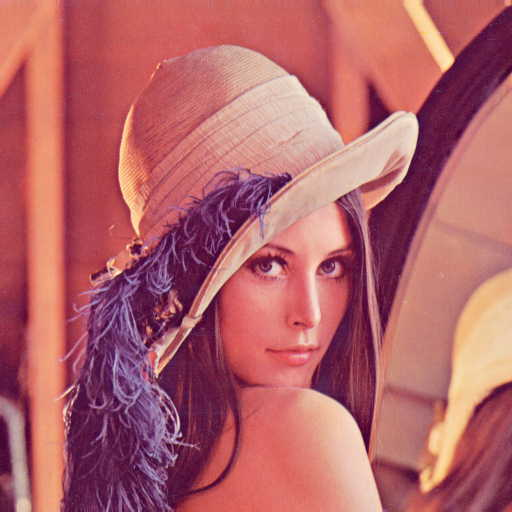
\includegraphics[width=0.7\textwidth]{lena.jpg}
\centering
}

\blindtext
\section{Verweise}
Mit \textbackslash ref und \textbackslash pageref können Verweise auf andere Kapitel bzw. Seiten erstellt werden. \emph{Kapitel und Unterkapitel} ist Kapitel \ref{kapitelunterkapitel} auf Seite \pageref{kapitelunterkapitel}.

\blindtext[2]

\section{Literaturverzeichnis}
Wie Tobias Oetiker \cite{lshort} schreibt, verwendet man \textbackslash cite um Literaturverweise und \textbackslash bibitem um das Literaturverzeichnis zu erstellen. Die \textbackslash bibitem Kommandos können dabei an einem beliebigen Ort, z.B. in einer separaten Datei oder am Ende des Dokuments stehen.

\begin{thebibliography}{99}
\bibitem{lshort} T. Oetiker:
\emph{The not so short introduction to \LaTeX{}}, Version 5.01, 2011
\bibitem{diePokerschule} Jan Meinert:
\emph{Die Pokerschule}, 2007 Kanaur Verlag, 2018 Droemer Verlag
\bibitem{MonteCarloSimulation} riskNET.de:
\emph{https://www.risknet.de/wissen/rm-methoden/monte-carlo-simulation/}, 10.2019
\end{thebibliography}

\end{document}
© 2019 GitHub, Inc.
Terms
Privacy
Security
Status
Help
Contact GitHub
Pricing
API
Training
Blog
About
